\documentclass[a4paper,12pt,twocolumn]{article}

%***************** Packages for Graphics & Figures *******************%
\usepackage{graphicx} %%For loading image files
\graphicspath{ {images/} } %folder-location for images

\usepackage{amsmath}

\newcommand*{\MyPath}{../latex-files}%

\begin{document}

\begin{abstract}

This paper presents the concepts and analysis of mass-spring damper system.  \cite{scipy}
 
\end{abstract}

\section{Introduction}
In this paper we will model a simple behaviour of mass-spring damper system and anaylsze system reponses.  Figure \ref{fig:block_diag} Shows an mass-spring damper system. 

\begin{figure}[!h]
\centering
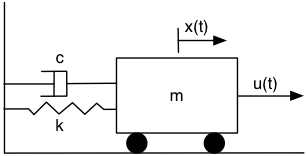
\includegraphics[scale = 0.6]{block_diag}
\label{fig:block_diag}
\caption{Mass Spring Damper System}
\end{figure}

Mass 'm' is attached to a spring, property of which is governed by Hooke's Law. $F_s = -k*x$, where k is called Spring Constant, $F_s$ is restoring force applied by spring and x is distance by which string is compressed or stretched.  Another component of system is a damper. Suppose we apply a force, say F in a direction, damper will apply a counter force in opposite direction. Therefore, damper acts as kind of shock absorber. 

\begin{figure}[!h]
\centering
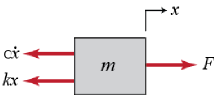
\includegraphics[scale = 0.6]{fbd}
\label{fig:fbd}
\caption{Free Body Diagram}
\end{figure}

We can use free body diagram to balance the force applied on body. As shown in Figure \ref{fig:fbd} and Figure \ref{fig:Response} \
\begin{equation}
 m \ddot{x} = u(t) - c \dot{x} - kx
 \label{equ:diff_equ}
\end{equation}

where: \\
x : position of mass [m] at time t seconds \\
m : mass of body [Kg] \\
c : viscous damping coefficient [Ns/m] \\
k : spring constant [N/m] \\
u : force input [N] \\

Rearranging equation \ref{equ:diff_equ} we can write 
\begin{equation}
  u(t) = m \ddot{x} + c \dot{x} + kx
 \label{equ:diff_equ_rearranged}
\end{equation}

Depending on the values of m, c, and k, the system can be underdamped, overdamped or critically damped. For each case the behaviour of the system will be different.

Equation \ref{equ:diff_equ_rearranged} is a $2^{nd}$ order differential equation. We will use state-space representation technique to analyze the system. State-space representation is choosen because it leds to first order differential equation and hence make analysis easier.

From $2^{nd}$ order differential of Equation \ref{equ:diff_equ_rearranged},we rename the dependent variable x and its first derivative as follows: \\
  \[ x_1(t) = x(t) \] 
  \[ x_2(t) = \dot{x}(t) = \dot{x_1}(t) \] 
  
where: \\
$x_1$ : position of the mass m \\
$x_2$ : derivative of $x_1$ = velocity of the mass (in m/s)

Just from this change of variables we get the first 1st order ode.
\begin{equation}
\dot{x_1}(t)=x_2(t)
\label{equ:x1}
\end{equation}

Substituting into the Equation \ref{equ:diff_equ} and noting that:
\[\dot{x_2}(t)=\ddot{x}(t)\]

we get:
\begin{equation}
m \dot{x_2} + c {x_2} + k x_1 = u
\end{equation}

\begin{equation}
\dot{x_2} = - (c/m) {x_2} - (k/m) x_1 + (1/m) u  
\label{equ: x2}
\end{equation}

Representing Equation \ref{equ: x1} and Equation \ref{equ: x2} in matrix form, we get:

\[
\begin{bmatrix} 
	\dot{x_1}\\ \dot{x_2} 
\end{bmatrix} = 
\begin{bmatrix} 
	0 & 1 \\ 
	- k/m &-c/m 
\end{bmatrix} 
\begin{bmatrix} 
	x_1\\x_2 
\end{bmatrix} + 
\begin{bmatrix} 
	0\\
	1/m 
\end{bmatrix} u  
\]
  
Also the output equation which represent the postion of the mass is :
\[
	y = 
	\begin{bmatrix} 
		{1}&{0} 
	\end{bmatrix} 
	\begin{bmatrix} 
		{x_1}\\ {x_2} 
	\end{bmatrix}   
\]

 
  
  
\begin{figure}
\centering
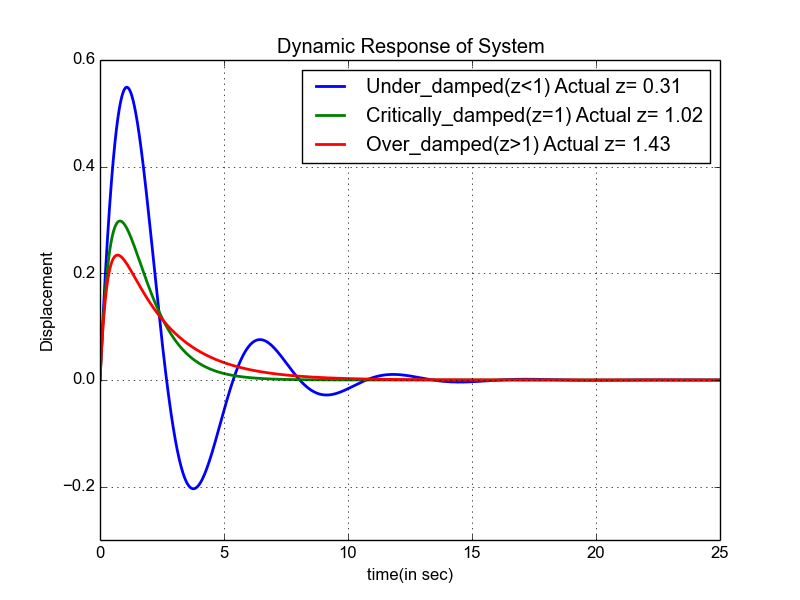
\includegraphics[scale = 0.5]{Response}
\label{fig:Response}
\caption{Dynamic Response of System for various values of damping coefficients}
\end{figure}


%  Bibilography
\bibliographystyle{plain}
\bibliography{\MyPath/references/references_LV_model.bib}

\end{document}
